\documentclass[11pt,letter]{article}
\usepackage[top=0.65in,bottom=0.9in,left=0.85in,right=0.85in]{geometry}

%\def\baselinestretch{1.25}
\def\baselinestretch{1.0}

\usepackage[greek, english]{babel}
\usepackage{multicol}

\usepackage{graphicx}
\usepackage[export]{adjustbox}


% The use of the times package forces the use of the type-1 times
% roman font, but the times roman font does not look nice.
% Besides the times roman font still does not print correctly on
% the dopy printer.
%\usepackage{times}


\usepackage{fancyhdr}
\usepackage{amsmath}
\usepackage{bm}
\usepackage{bbold}
\usepackage{parskip}

\newcommand{\bv}[1]{\ensuremath{\bm{#1}}}
\newcommand{\Lc}{\ensuremath{L_{\mathrm{c}}}}
\newcommand{\dsig}[1]{\ensuremath{ \frac{ d\,\sigma_{#1} }{d\,\Omega} }}

\begin{document}

\section{Data with Debye-Waller factor correction for direct comparisson with QMC} 
Our QMC collaborators compute $S(\bv{Q})$, which is related to our measurement as 
\begin{equation}
 I(t) = I_{\mathrm{TOF}=\infty}( 1 +  DW_{t}( S(\bv{Q}) - 1 ) )
\end{equation}
where $DW_{t}$ is the TOF dependent Debye-Waller factor.
 Previously
we presented our collaborators the data  which did not have a Debye-Waller
factor correction.   Here we make a correction, also noting that we only made
measurements in situ and at $t=6\mu\mathrm{s}$ .   With these two measurements one can
solve for the spin structure factor 
\begin{equation}
 I_{t} \equiv \frac{ I(t=0)}{I(t)} = \frac{ 1 + DW_{0}(S(\bv{Q})-1) }{ 1 + DW_{t}(S(\bv{Q})-1)} 
\end{equation}
\begin{equation}
\Rightarrow S(\bv{Q}) = \frac{  I_{t}(1-DW_{t}) - (1-DW_{0})}{ DW_{0} - I_{t}DW_{t} } 
\end{equation}
In the long time limit ($DW_{t}=0$), and for negligible wavefunction size in the lattice ($DW_{0}=1$) this reduces to $S(\bv{Q})=I_{t}$. 

The data including this Debye-Waller factor correction is shown in Fig.~\ref{fig:data} and also attached to the email.
\begin{figure}
\centering 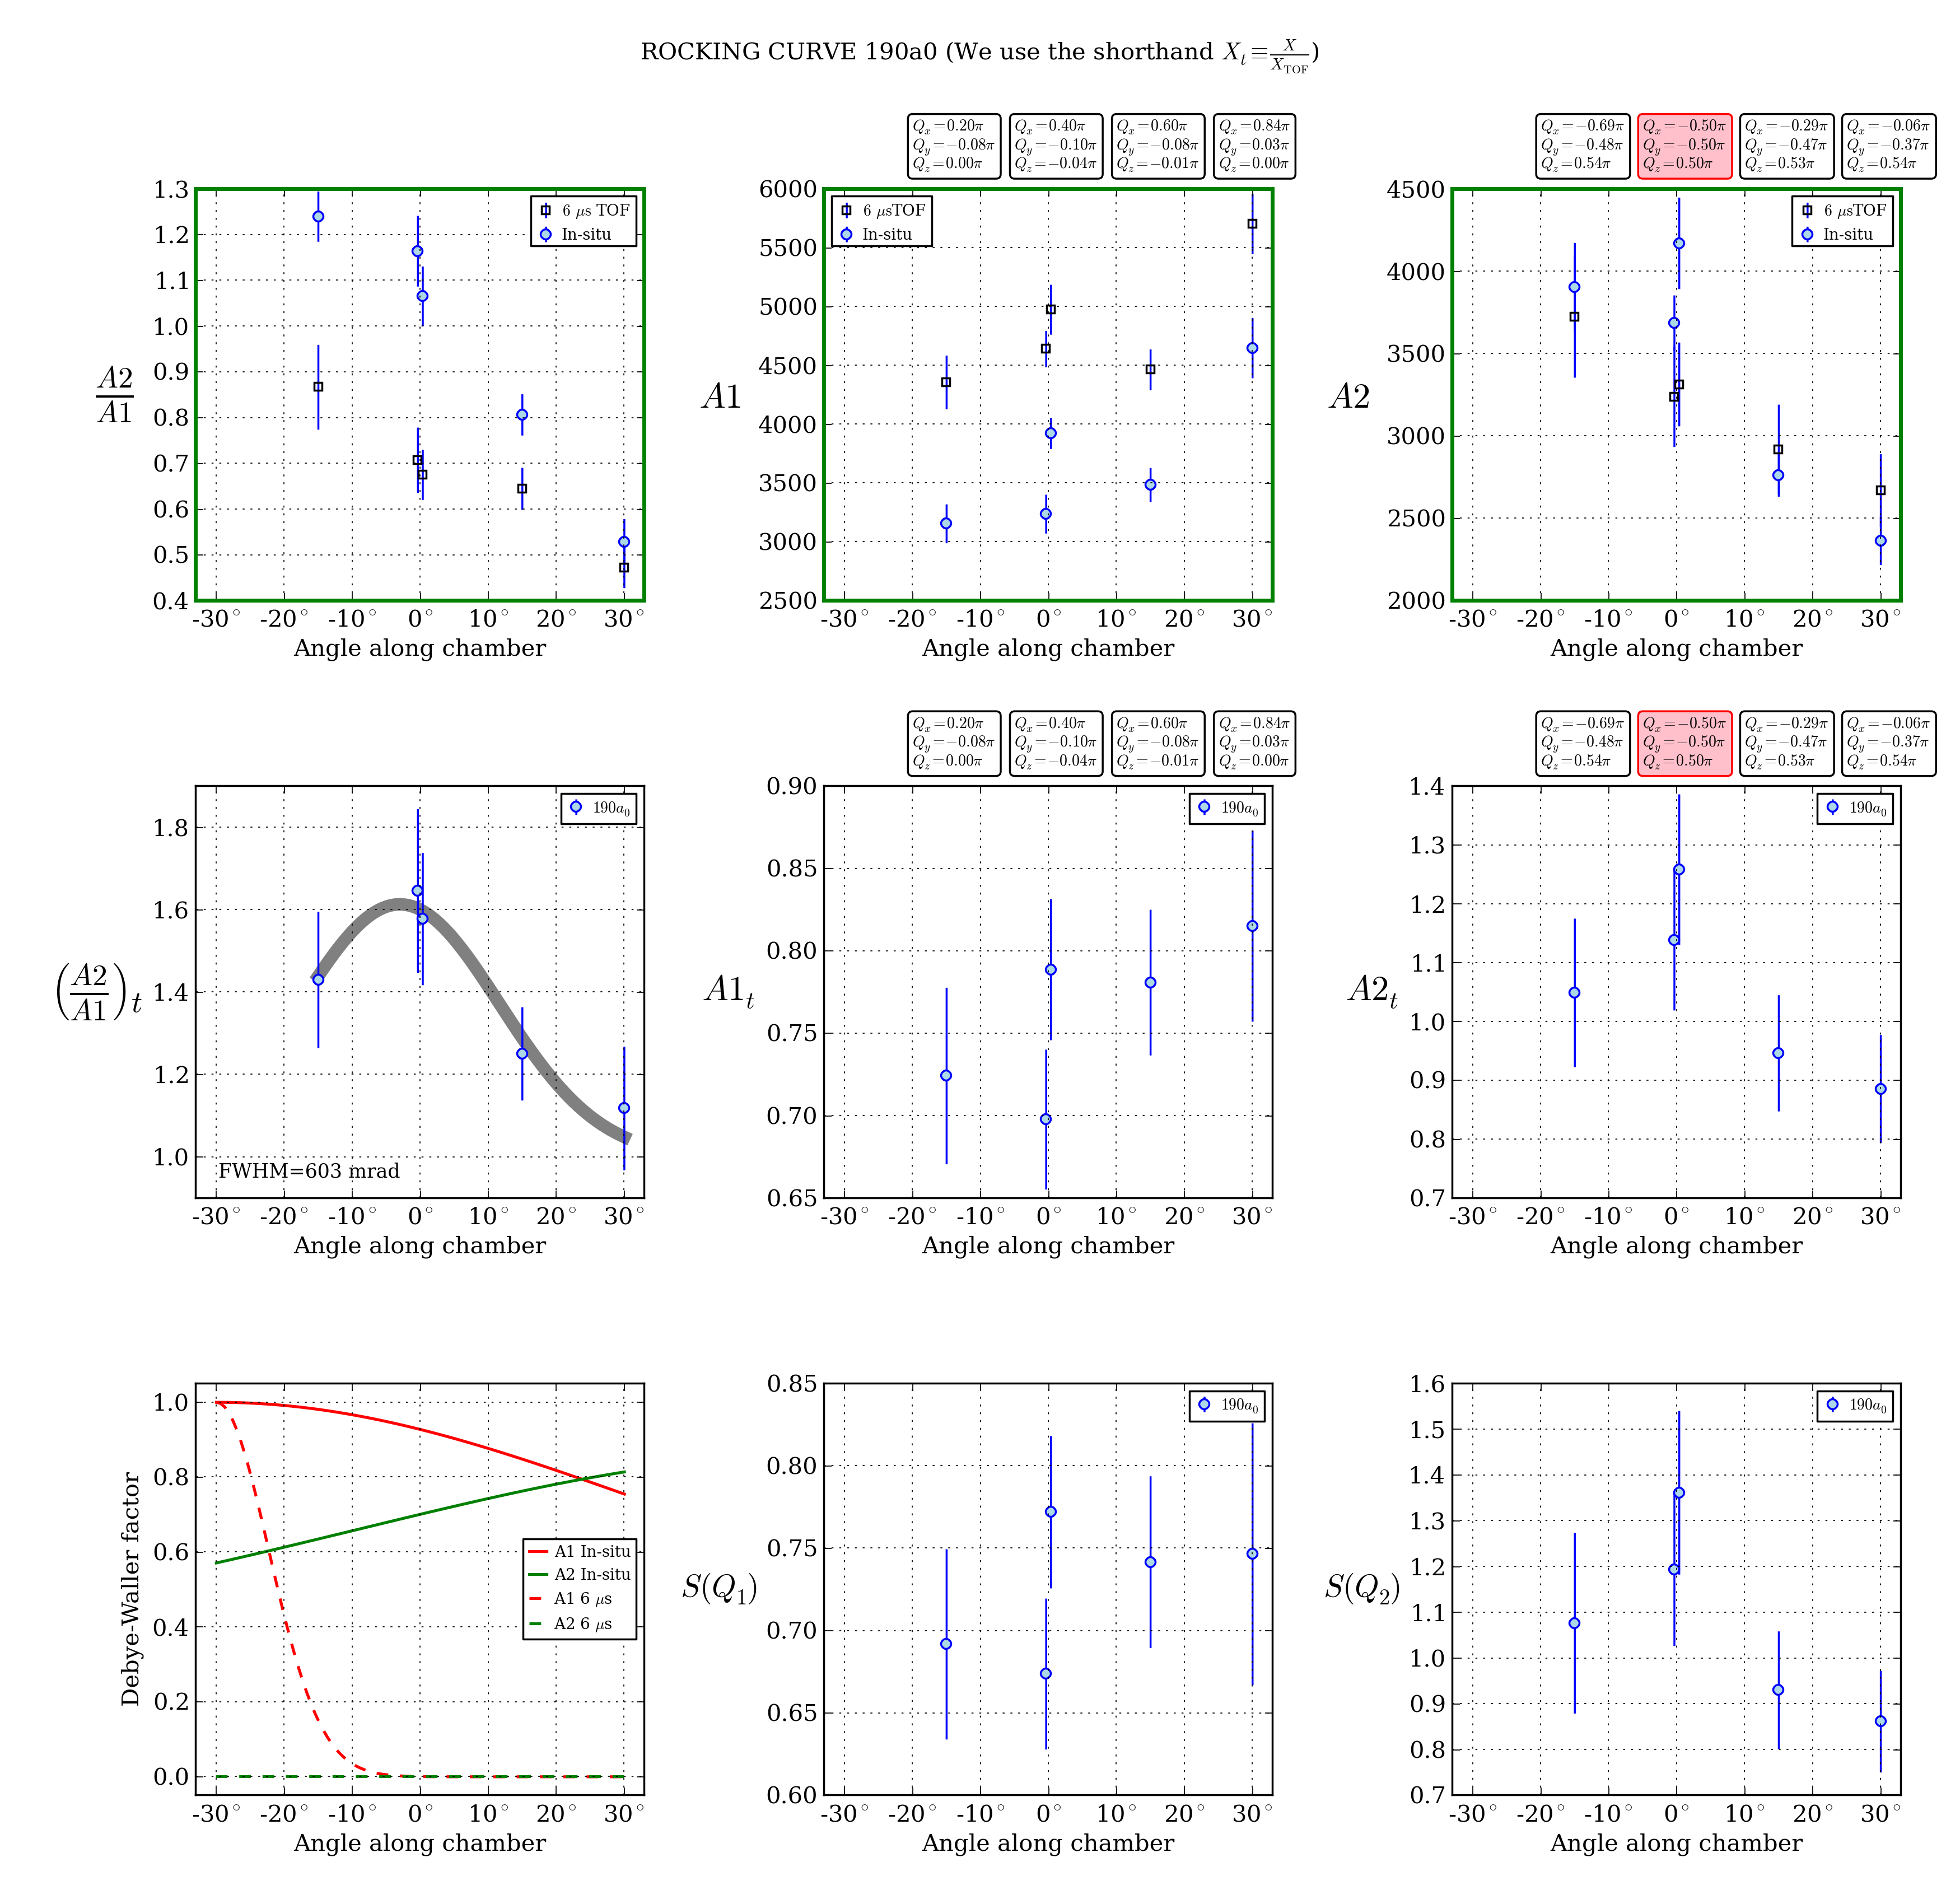
\includegraphics[width=\textwidth]{figures/rocking.png}
\caption[Rocking at 190$a_{0}$]{\small Top row shows our raw data, which corresponds to ratio of CCD counts $A2/A1$, and CCD counts for $A1$, $A2$ respectively.  Middle row shows the ratio of in-situ and TOF data for each of the three quantities.  Bottom row, left panel shows the Debye-Waller factor for the in-situ picture and the 6~$\mu$s TOF picture as a function of angle along chamber.  The $A1$ Debye-Waller factor goes to 1 for both in-situ and TOF at 30$^{\circ}$, which corresponds to zero momentum transfer.  Bottom row, right panels show the spin structure factor determined from our data and the Debye-Waller factor corrections. }
\label{fig:data}
\end{figure}


 

%\bibliographystyle{osa}
%\bibliography{refs}

\end{document}




